\documentclass[10pt,conference,a4paper]{IEEEtran}

%import packages here
\usepackage{amsmath}
\everymath{\displaystyle}
\usepackage{graphicx}
\usepackage{caption}
\graphicspath{{Images/}}

\title{Lucky Thirteen - A Cryptographic Analyses}
\author{Ruud Verbij \\ Student at the University of Twente \\ crypto@ruudverbij.nl}
\begin{document}
\maketitle

\begin{abstract}

\end{abstract}

\begin{IEEEkeywords}
Cryptography, SSL, TLS, Lucky Thirteen, Padding Oracle, Timing attacks
\end{IEEEkeywords}

\section{Introduction}
\label{sec:intro}

\section{Short overview of Cryptography in TLS}
\label{sec:crypto}

\section{Padding Oracle Attacks}

\label{sec:paddingoracle}
\subsection{}

\subsection{Bomb Oracles}
\label{sec:paddingoracle:bomb}
blabla $\oplus$ blabla

\section{TLS}
\label{sec:TLS}
TLS 1.1 and 1.2: check the padding format carefully, report a single error message for padding and MAC failures, and make the record processing time essentially the same whether or not the padding is correct.

\begin{figure}[h]
	\centering
	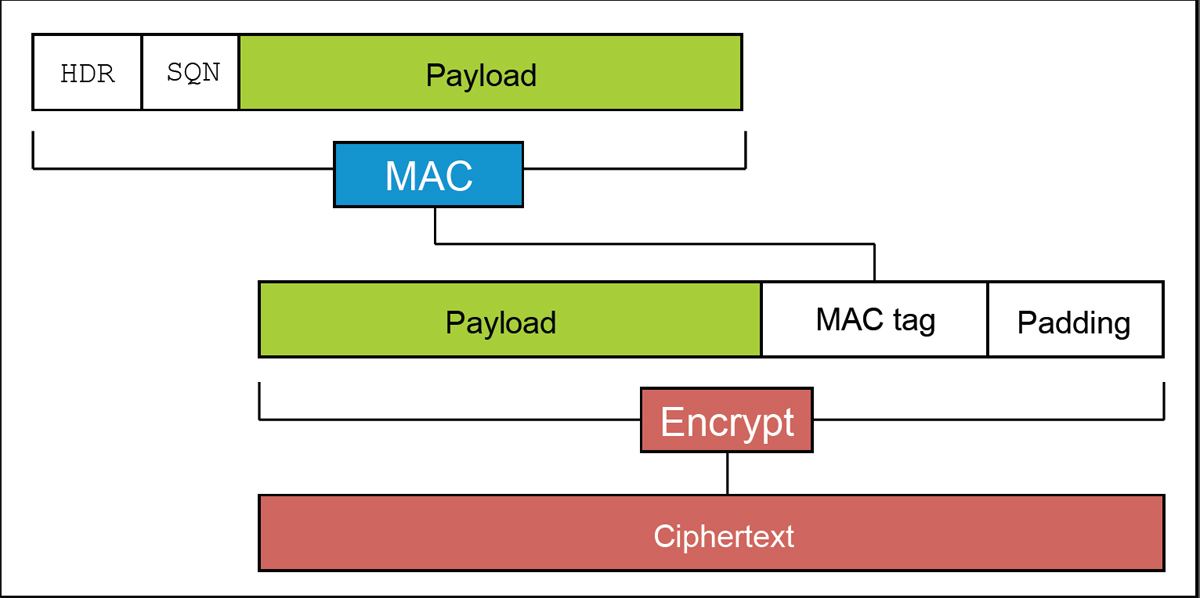
\includegraphics[width=0.5\textwidth]{tls-representation.jpg}
	\caption{Representation of TLS~\cite{alfardan2013lucky}}
	\label{fig:tls}
\end{figure}

\section{Lucky Thirteen}
\label{sec:lucky}
regular plaintext recovery of a block: 2\^23 connections
if base64 (cookies, http basic access authentication) used: 2\^23 -> 2\^19 connection per block
per cookie byte, using BEAST technique: 2\^13 connections

\section{The Future of TLS}
\label{sec:future}

\bibliographystyle{IEEEtran}
\bibliography{IEEEabrv,literature}
\end{document}






























